\documentclass[runningheads]{llncs}
%\documentclass[a4paper]{llncs}
%\usepackage[spanish,es-noshorthands,es-tabla]{babel}
%\renewcommand\spanishtablename{Otro nombre}
%\renewcommand\keywordname{{\bf Palabras clave:}}
\usepackage{amssymb}
\setcounter{tocdepth}{3}
\usepackage{graphicx,epsfig}
\usepackage{algorithmic}
\usepackage{listings}
\usepackage{rotating}
\usepackage{subfig}
\usepackage{listings}
%%%%

\usepackage{courier}
\usepackage{color}
\usepackage{alltt}
\usepackage{verbatim}
\usepackage{url}
\usepackage[utf8]{inputenc}

\usepackage{array}

\usepackage{url}

\newcommand{\keywords}[1]{\par\addvspace\baselineskip
\noindent\keywordname\enspace\ignorespaces#1}

\lstset{
basicstyle=\ttfamily \scriptsize,
language=c++,
frame=single,
stringstyle=\ttfamily,
showstringspaces=false
}

\renewcommand{\textfraction}{0}
\renewcommand{\topfraction}{1}
\renewcommand{\bottomfraction}{1}
\renewcommand{\floatpagefraction}{0.9}

\begin{document}

\mainmatter  % start of an individual contribution

% first the title is needed
\title{Adapting parallel evolutionary algorithms to concurrent and functional paradigms}

\author{J. Albert-Cruz\inst{1}, J.J. Merelo\inst{2}, L. Acevedo-Martínez\inst{1}}

\titlerunning{Adapting evolutionary algorithms to concurrent languages}

\authorrunning{J. Albert Cruz et al.}

\institute{
Centro de Estudios de Matem\'atica Computacional, Universidad de Ciencias Inform\'aticas, Cuba
\and Dept. Arquitectura y Tecnología de los Computadores, Universidad de Granada, España \\ jalbert@uci.cu}

%\tocauthor{Authors' Instructions}

\maketitle

\begin{abstract}
The current multi-core microprocessor's architecture challenge the entire software industry, to take advantage of them is necessary a parallel implementation of every simple program. Concurrent programming is hard; to use programming languages with built-in concurrent concepts is one way to face that. This work describes the design and implementation of an evolutionary computation model using the concurrent and functional paradigms of programming in the languages Erlang, Scala y Clojure. This article shows the advantages of these paradigms in order to implement a hybrid parallel genetic algorithm with an island topology. Some design decisions are analyzed and the results of the solution of a case study are showed.
\end{abstract}

\keywords{Evolutionary Algorithms, Functional Languages, Concurrent Languages, Implementation, Modeling}


\section{Introduction}
\label{sec:intro}
    
\noindent Genetic algorithms (GA) \cite{GA_Goldberg89} are currently one of the most used meta-heuristics to solve engineering problems. Furthermore, parallel genetic algorithms (pGAs) are useful to find  solutions of complex optimizations problems in adequate times \cite{Luque2011}; in particular, problems with complex fitness. Some authors \cite{Alba2001} state that using pGAs improves the quality of solutions in terms of the number of evaluations needed to find one. This reason, together with the improvement in evaluation time brought by the simultaneous running in several nodes, have made parallel and distributed evolutionary algorithms a popular methodology.

Running evolutionary algorithms in parallel is quite straightforward, but programming paradigms used for the implementation of such algorithms is far from being an object of study. Object oriented or procedural languages like Java and C/C++ are mostly used. Even when some researchers show that implementation matters \cite{DBLP:conf/iwann/MereloRACML11}, parallels approaches in new languages/paradigms is not normally seen as a land for scientific improvements.

New parallel platforms have been identified as new trends in pGAs \cite{Luque2011}, however only hardware is considered. Software platforms, specifically programming languages, remain poorly explored; only Ada \cite{Santos2002} and Erlang \cite{A.Bienz2011,Kerdprasop2013} were slightly tested.

%The multicore’s challenge \cite{SutterL05} shows a current need for making parallel even the simplest program. But this way leads us to use and create design patterns for parallel algorithms; the conversion of a pattern into a language feature is a common practice in the programming languages domain, and sometimes that means a language modification, others the creation of a new one.

This work explores the advantages of some non mainstream languages (not included in the top ten of any most popular languages ranking) with concurrent and functional features in order to develop GAs in its parallel versions. It is motivated by the lack of community attention on the subject and the belief that using concepts that simplify the modeling and implementation of such algorithms might promote their use in research  and in practice.

This research is intended to show some possible areas of improvement on architecture and engineering best practices for concurrent-functional paradigms, as was made for Object Oriented Programming languages \cite{EO:FEA2000}, by focusing on pGAs as a domain of application and describing how their principal traits can be modeled by means of concurrent-functional languages constructs. We are continuing the research reported in 
other papers (hidden for double-blind review).
%\cite{DBLP:conf/gecco/CruzGGC13,J.Albert-Cruz2013}.

The rest of the paper is organized as follows. Next section presents the state of the art in concurrent and functional programming language paradigms and its potential use for implementing pGAs. Our proposal to adapt pGAs to the paradigms using a study case is explained in section \ref{sec:impl} as well as the experimental results in section \ref{sec:results}. In section \ref{sec:sample} we show a sample program of canonical island/GA implemented in Scala.

Finally, we draw the conclusions and future lines of work in section \ref{sec:conclusions}.



\section{Paradigms}
\label{sec:paradigmas}
    
Develop correct software quickly is a never ending goal in the software industry. There are two no-mainstream programming paradigms: the functional and the concurrent, trying to make a difference providing new abstraction tools. The functional languages are available since a long time (LISP is a very old programming language) nevertheless their use has been limited mainly for the inefficiency of theirs compilers or interpreters. Currently these situations have change, the problems solved and the advantages have promoting the inclusions of several functional concepts in modern and mainstream languages, C\# for example, or even the creation of new ones (Clojure).

Among the emergent languages with the concurrent paradigm excels Clojure, Go, Scala, Haskell and Erlang \cite{Nov.-Dec.2012}; they have built-in programming constructs for manage concurrency simplifying his correct use. 

\subsection{Concurrent programming}
    
El paradigma de programación concurrente, o como lo acuñara Joe Armstrong en \cite{Armstrong2003}: la {\em programación orientada a concurrencia} se caracteriza, en los lenguajes que la soportan, por la presencia de construcciones para el procesamiento de procesos (unidades de ejecución de código) que les dan el mismo tratamiento que a cualquier otro dato.

A la hora de desarrollar aplicaciones concurrentes el problema mayor a resolver es el de la comunicación entre procesos. Entre
los esfuerzos por formalizar y simplificar dicha actividad se encuentra el {\em Communicating Sequential Processes} de Hoare \cite{Hoare:1978:CSP:359576.359585}, dicho lenguaje de descripción de patrones de interacción ha servido de base para la creación de nuevos lenguajes de programación o librerías.


To be continued...

\subsection{Functional programming}
    El paradigma de la programación funcional por su parte, aún cuando ofrece varias ventajas, no ha sido muy usado. Un tiempo atrás se exploraron en el campo de la Programación Genética \cite{Briggs:2008:FGP:1375341.1375345,Huelsbergen:1996:TSE:1595536.1595579,walsh:1999:AFSFESIHLP}, más recientemente en la neuroevolución  \cite{Sher2013}; sin embargo dentro de los AG ha sido poca su presencia \cite{Hawkins:2001:GFG:872017.872197}.

La programación funcional se caracteriza por el uso de las funciones como datos (pasándolas por parámetros y devolviéndolas como resultados), en particular de las funciones puras: aquellas cuyo resultado solo depende de los parámetros de entrada, excluyendo los cambios de estado. Esto la hace particularmente adecuada para el desarrollo de algoritmos concurrentes pues estos tienen la primera fuente de errores y complejidad en la comunicación entre procesos, a través de cambios de estado.

El uso de listas, con implementaciones muy eficientes, es omnipresente en la programación funcional; en los AGs por su parte es una de las estructuras de datos más utilizadas, lo cual facilita el proceso de implementación de los diversos modelos de algoritmos evolutivos.



\section{Multi-paradigms emergent languages}
\label{sec:emergentes}
    
The field of programming languages research is very active in the Computer Science discipline. To find software construction tools with new and better means of algorithms expression is well welcome. In the last few years the functional and concurrent paradigms have been produced a rich mix in which concepts of the first one had been simplified the use of the second one.

%Esta sección es un poco corta...

%\subsection{Lenguaje Erlang}
%    
Erlang es un lenguaje de programación funcional, concurrente y
distribuido, adecuado para la construcción de sistemas que requieran grandes niveles de distribución \cite{veldstra:_welcom_erlan}, tolerancia a fallos y disponibilidad. Ha sido en más de una ocasión escogido por encima de C/C++ para el desarrollo de sistemas de uso intensivo de recursos \cite{Cesarini2009} dada la eficiencia de su ejecución \cite{erlang:future}. 

Utiliza el modelo {\em actor} para su implementación del paradigma de programación concurrente y posee facilidades para la integración con otros lenguajes tales como C/C++ y Java. Sus procesos son manejados por su máquina virtual (MV), que tiene un planificador por cada núcleo de la CPU, lo cual lo hacen ideal para la actual (y venideras) generación de procesadores multi-núcleos.

El que sea un lenguaje concurrente significa que posee entre sus tipos de datos el de proceso, en vez de ser facilidades proveídas por bibliotecas como en la mayoría de los lenguajes. Siendo en principio tan ligeros que una misma instancia de la MV puede tener millones en ejecución.
%
%\subsection{Lenguaje Scala}
%    
Scala es un lenguaje de programación estáticamente tipado, que integra conceptos del paradigma funcional con el orientado a objetos y posee un sistema de tipos lo suficientemente expresivo como para {\em escalar} (extenderse) mediante bibliotecas.

A partir del éxito obtenido por Erlang en el uso del concepto de actor para manejar la concurrencia se ha proveído a la biblioteca estándar del lenguaje con una implementación de actores que recientemente ha decidido cambiarse por la presente en la biblioteca Akka.


To be continued...

%
%\subsection{Lenguaje Clojure}
%    
Clojure es un lenguaje de programación dinámicamente tipado, que integra conceptos del paradigma funcional y el concurrente. Como parte de la herencia de los Lisp posee un sistema de macros que le da un alto nivel de extensibilidad.

Ha sido desarrollado con la idea de aprovechar la JVM proveyendo conceptos de alto nivel para el desarrollo de aplicaciones concurrentes.

To be continued...


\section{A functional-concurrent approach to GAs}
\label{sec:design}
    
In order to design the architecture of a software in the GAs application domain, we mostly identify the main concepts involved and the relations among them. Then, using the concepts of the paradigms and programming techniques chosen, we define the structure from the highest levels of abstraction indicating the data to be processed and their flow. The quality and extensibility of that structure might determine the succeed or failure of the software.

The main GA’s components identified in that work for designing our proposal are listed in Table \ref{agpComp}.

\begin{table}
  \centering
  \caption{Parallel GA's components.}\label{agpComp}
   \begin{tabular}{|>{\centering}p{3cm}|p{5cm}|p{3cm}|}
   \hline
   \textbf{AG Component} & \textbf{Rol} & \textbf{Description} \\
     \hline
      chromosome & Representing the solution. & binary string \\
     \hline
      evaluated chromosome & Pair \{chromosome, fitness\}. & relation thats indicate the value of a individual\\
     \hline
      population & Set of chromosomes. & list \\
     \hline
     crossover & Relation between two chromosomes producing other two new ones. & crossover's function \\
     \hline
      mutation & A chromosome modification. & chromosome's change function \\
     \hline
     selection & Means of population filtering. & selection's function \\
     \hline
      pool & Shared population among node's calculating units. & population \\
     \hline
      island & Topology's node. &  \\
     \hline
      migration & Random event for chromosome interchange. & message \\
     \hline
      evolution & Execution. & A generation is made \\
     \hline
      evaluation & Execution. & A fitness calculi is made \\
     \hline
   \end{tabular}

\end{table}

On the other hand, to develop an optimal codification of an algorithm is mandatory to know every characteristic of the programming language in use.

In this work we used hybrid pGAs: an island topology with a pool based pGA in each node. We chose the {\em Max-SAT} problem with 100 variable instances \cite{Hoos2000}.


\section{Implementations}
\label{sec:impl}
    
With the initial domain analysis and using the concurrent and functional concepts properly, the following design and implementation were conceived. 

\subsection{Erlang modeling}
    \begin{table}
  \centering
   \caption{Construcciones de Erlang.}\label{erlComp}
\begin{tabular}{|p{3.4cm}|p{7cm}|}
  \hline
  % after \\: \hline or \cline{col1-col2} \cline{col3-col4} ...
  \textbf{Concepto Erlang} & \textbf{Papel} \\
     \hline
  tupla & Tipo de datos para representar entes compuestos cuyas componentes sean de diferentes tipos y no varíen en el tiempo. \\
     \hline
  lista & Tipo de datos para representar entes compuestos cuyas componentes sean de igual tipo y varíen en el tiempo.\\
     \hline
  función & Relaciones entre datos, operaciones. \\
     \hline
  actor & Unidad de ejecución, proceso. \\
     \hline
  mensaje & Comunicación entre actores. \\
     \hline
  ets & Listado de cromosomas compartidos mediante el pool. \\
     \hline
  módulo random & Generación de números aleatorios.\\
  \hline
\end{tabular}

\end{table}

\begin{table}
  \centering
  \caption{Mapeo entre conceptos de Erlang y de AGs.}\label{erlAGRelation}
\begin{tabular}{|p{3cm}|p{6cm}|}
  \hline
  % after \\: \hline or \cline{col1-col2} \cline{col3-col4} ...
  \textbf{Concepto Erlang} & \textbf{Concepto AG en el que se emplea} \\
     \hline
  tupla & cromosoma evaluado \\
     \hline
  lista & cromosoma y población \\
     \hline
  función & cruzamiento, mutación y selección \\
     \hline
  actor  & isla, evaluador y reproductor \\
     \hline
  mensaje & migración \\
     \hline
  ets & pool \\
     \hline
  módulo random & naturaleza estocástica del AG \\
  \hline
\end{tabular}

\end{table}

Los principales conceptos concurrentes y funcionales utilizados son: actor, mensaje, función y lista. Su uso en la implementación de la arquitectura híbrida utilizada se basó en la flexibilidad y rapidez de implementación que permitiera. Para los procesos independientes existentes, ya fueran las islas o los evaluadores y reproductores se emplearon actores; para la comunicación entre ellos se usaron mensajes al ser estos el concepto indicado para comunicar actores. La lógica de funcionamiento del AG se expresó en funciones (medio funcional para la transformación de los datos) y las unidades de datos (cromosomas, poblaciones y configuraciones) se codificaron en listas y tuplas que son las estructuras de datos básicas del paradigma funcional.




\subsection{Library erlEA}
    En la realización del caso de estudio fue implementado, teniendo en cuenta los conceptos seleccionados anteriormente, un proyecto Erlang de varios módulos. El código se encuentra bajo la licencia AGPL, de código abierto, en la dirección: \url{https://github.com/jalbertcruz/erlEA/tree/book2013}. Sus principales módulos y funciones son descritos a continuación.


\subsubsection{Módulo reproducer}

Este es el módulo que selecciona la subpoblación a reproducir, los padres, realiza el cruzamiento y desencadena las migraciones. Como actor responde a los mensajes {\em evolve}: para realizar una iteración y {\em emigrateBest} para efectuar una emigración. Las funciones con las que logra esto aparecen enumeradas en la Tabla \ref{tb:reproducer}.

\begin{table}
  \caption{Funciones del módulo reproducer.}\label{tb:reproducer}
  \centering
\begin{tabular}{|p{5cm}|p{7cm}|}
  \hline
  % after \\: \hline or \cline{col1-col2} \cline{col3-col4} ...
   \textbf{Función} &  \textbf{Descripción} \\
  \hline
  {\tt extractSubpopulation(Table, N) } & A partir de una {\em ets} y una cantidad, selecciona de la {\em ets} un grupo de cromosomas. \\
  \hline
  {\tt bestParent(Pop2r)} & Selecciona de una lista de cromosomas el mejor individuo. \\
  \hline
 {\tt selectPop2Reproduce(Pop, N)} & Selecciona aleatoriamente un conjunto de pares de una lista de cromosomas. \\
  \hline
  {\tt crossover(Ind1, Ind2)} & Realización de un cruce y mutación sobre el mismo, a partir de dos cromosomas. \\
  \hline
\end{tabular}
\end{table}


\subsubsection{Módulo evaluator}

Este es el módulo que calcula el fitness: hace periódicas consultas sobre el pool para obtener individuos a los que calcularle el fitness. Está compuesto por la función {\em SatMax/1} (función de evaluación), y por el mensaje {\em eval}, dicho mensaje es el que activa al evaluador para que calcule.

\subsubsection{Módulo poolManager}

Este es el módulo encargado de inicializar el trabajo del pool así como enrutar los mensajes entre los evaluadores. Es el encargado de controlar la finalización del algoritmo una vez se ha encontrado la solución.  Los mensajes a los que responde este actor aparecen enumerados en la Tabla \ref{tb:poolManager}.

\begin{table}
  \caption{Mensajes a los que responde el actor del módulo poolManager.}\label{tb:poolManager}
  \centering
\begin{tabular}{|p{3cm}|p{7cm}|}
  \hline
  % after \\: \hline or \cline{col1-col2} \cline{col3-col4} ...
   \textbf{Mensaje} &  \textbf{Descripción} \\
  \hline
  {\tt evolveDone } & Finalización de una iteración de reproducción. \\
  \hline
  {\tt evalDone} & Finalización de una iteración de evaluación. \\
  \hline
 {\tt solutionReached} & Obtención de la solución. \\
  \hline
  {\tt migration} & Realización de una inmigración. \\
  \hline
\end{tabular}
\end{table}


\subsubsection{Módulos auxiliares e interconexión}

Los módulos ya descritos contienen toda la lógica del AG, faltan sin embargo, para que sea operativo el software, algunos componentes no funcionales.

\vspace{.35cm}

\noindent  Dichos componentes son:
\begin{description}

  \item[experiment] -- Encargado de iniciar una corrida del experimento.

  \item[configBuilder] -- Especificación de los parámetros de un experimento.

  \item[profiler] -- Análisis del comportamiento: tiempos de ejecución, cantidad de iteraciones, etc.

  \item[manager] -- Control del inicio y coordinación de la finalización adecuada de cada unidad de ejecución durante la corrida de un experimento.

  \item[report] -- Control de la secuencia de experimentos y emisión del reporte final resultado de la experimentación.

\end{description}

\noindent Los diferentes módulos interactúan de la siguiente manera durante una sesión de experimentación:

\begin{enumerate}

  \item Configuración de los parámetros: tamaño de población y cromosomas, población inicial, conformación de la topología de las islas. Módulos {\em experiment} y {\em configBuilder}.

  \item Lógica del AG: reproducción, selección de padres, emigraciones, cálculo del fitness. Módulos {\em evaluator} y {\em reproducer}.

  \item Control del proceso y reportes: enruteo de mensajes entre islas y unidades de ejecución (actores), coordinación de los procesos de finalización de una corrida e inicio de otra, resumen y formateo de salida de los resultados. Módulos {\em poolManager}, {\em profiler}, {\em manager} y {\em report}.

\end{enumerate}


\subsection{Scala modeling}
    
En el caso de la implementación en Scala se siguieron las mismas pautas que en el caso de Erlang al ser el mismo patrón (actor) el presente. Las diferencias están en el soporte de objetos de Scala y en el rendimiento al hacerse uso de la JVM.

To be continued...

\subsection{Library sclEA}
    
En la realización del caso de estudio fue implementado, teniendo en cuenta los conceptos seleccionados anteriormente, un proyecto Scala de varias clases. El código se encuentra bajo la licencia AGPL, de código abierto, en la dirección: \url{https://github.com/jalbertcruz/sclEA/tree/book2013}. Sus principales clases y funciones son descritas a continuación.


\subsubsection{Clase Reproducer}

Este es la clase que selecciona la subpoblación a reproducir, los padres, realiza el cruzamiento y desencadena las migraciones. Como actor responde a los mensajes {\em evolve}: para realizar una iteración y {\em emigrateBest} para efectuar una emigración. Las funciones con las que logra esto aparecen enumeradas en la Tabla \ref{tb:scl:reproducer}.

\begin{table}
  \caption{Funciones del módulo reproducer.}\label{tb:scl:reproducer}
  \centering
\begin{tabular}{|p{5cm}|p{7cm}|}
  \hline
  % after \\: \hline or \cline{col1-col2} \cline{col3-col4} ...
   \textbf{Función} &  \textbf{Descripción} \\
  \hline
  {\tt extractSubpopulation(pTable: HashMap[String, (Int, Int)], n: Int) } & A partir de una {\em ets} y una cantidad, selecciona de la {\em ets} un grupo de cromosomas. \\
  \hline
  {\tt bestParent(pop2r: List[(String, Int)]): (String, Int)} & Selecciona de una lista de cromosomas el mejor individuo. \\
  \hline
 {\tt selectPop2Reproduce(subpop: List[(String, Int)], parentsCount: Int)} & Selecciona aleatoriamente un conjunto de pares de una lista de cromosomas. \\
  \hline
  {\tt crossover(parents: ((String, Int), (String, Int))): (String, String)} & Realización de un cruce y mutación sobre el mismo, a partir de dos cromosomas. \\
  \hline
\end{tabular}
\end{table}


\subsubsection{Clase Evaluator}

Esta es la clase que calcula el fitness: hace periódicas consultas sobre el pool para obtener individuos a los que calcularle el fitness. Está compuesto por el método {\em SatMax/1} (función de evaluación), y por el mensaje {\em eval}, dicho mensaje es el que activa al evaluador para que calcule.

\subsubsection{Clase PoolManager}

Esta es la clase encargada de inicializar el trabajo del pool así como enrutar los mensajes entre los evaluadores. Es el encargado de controlar la finalización del algoritmo una vez se ha encontrado la solución.  Los mensajes a los que responde este actor aparecen enumerados en la Tabla \ref{tb:scl:poolManager}.

\begin{table}
  \caption{Mensajes a los que responde el actor de la clase PoolManager.}\label{tb:scl:poolManager}
  \centering
\begin{tabular}{|p{3cm}|p{7cm}|}
  \hline
  % after \\: \hline or \cline{col1-col2} \cline{col3-col4} ...
   \textbf{Mensaje} &  \textbf{Descripción} \\
  \hline
  {\tt evolveDone } & Finalización de una iteración de reproducción. \\
  \hline
  {\tt evalDone} & Finalización de una iteración de evaluación. \\
  \hline
 {\tt solutionReached} & Obtención de la solución. \\
  \hline
  {\tt migration} & Realización de una inmigración. \\
  \hline
\end{tabular}
\end{table}


\subsubsection{Clases auxiliares e interconexión}

Las clases ya descritas contienen toda la lógica del AG, para que sea operativo el software sin embargo, han de incluirse algunos componentes no funcionales.

\vspace{.35cm}

\noindent  Dichos componentes son:
\begin{description}

  \item[Objetos ExperimentRun y Experiment] -- Encargados de iniciar una corrida del experimento.

  \item[Clase Profiler] -- Análisis del comportamiento: tiempos de ejecución, cantidad de iteraciones, etc.

  \item[Clase Manager] -- Control del inicio y coordinación de la finalización adecuada de cada unidad de ejecución durante la corrida de un experimento.

  \item[Clase Report] -- Control de la secuencia de experimentos y emisión del reporte final resultado de la experimentación.

\end{description}

\noindent Los diferentes módulos interactúan de la siguiente manera durante una sesión de experimentación:

\begin{enumerate}

  \item Configuración de los parámetros: tamaño de población y cromosomas, población inicial, conformación de la topología de las islas. Objetos {\em Experiment} y {\em ExperimentRun}.

  \item Lógica del AG: reproducción, selección de padres, emigraciones, cálculo del fitness. Clases {\em Evaluator} y {\em Reproducer}.

  \item Control del proceso y reportes: enruteo de mensajes entre islas y unidades de ejecución (actores), coordinación de los procesos de finalización de una corrida e inicio de otra, resumen y formateo de salida de los resultados. Clases {\em PoolManager}, {\em Profiler}, {\em Manager} y {\em Report}.

\end{enumerate}


\subsection{Clojure modeling}
    The Clojure’s main concurrent concepts used are agent, ref and atom; the functional ones are function and list. Clojure is a language with a very strict control of state change; it demands a clear identification of the code doing it and that’s similar to Erlang where the functional purity is pursued too.

Agents were the concept used for implement the independent units of execution (reproductors, evaluators and islands). The communication between agents was made by protocol’s functions due to the flexibility need. GA’s operations, their logic and constraints, were express in functions and protocol’s implementations and the data was encoded in lists and vectors data structures. 

\subsection{Library cljEA}
    
We developed a library in Clojure following the same design concepts and it was tested with the case study. The code is open, under AGPL license, at \url{https://github.com/jalbertcruz/cljEA/tree/evostar2014}. This implementation uses the same naming and architectural convection as in Erlang and Scala.

\section{Case study application}
\label{sec:results}
    
All used languages have functional and concurrent built-in features, with the first ones supporting the second ones. Erlang and Scala’s implementations are based in the actor pattern for doing parallel computation. Clojure on the other hand works with the agent concept, a similar model with simplified ways of reading the involved information.

To communicate modules we used language’s dependent (different) data types. The message's structure was tuples for Erlang and Scala, and for agents it was necessary to encapsulate functions on protocols (Clojure variants of Java interfaces). For sharing individuals (the pool) we used functionals consult/modification data structures: hash-like for Scala/Clojure and the {\em ets} module in Erlang’s case. The data was encoded with compound data structures: lists, vectors, tuples, records, etc. The Table \ref{tb:res:comp} summarizes the differences between the languages.

\begin{table}
  \caption{Language's comparisons.}\label{tb:res:comp}
  \centering
  \begin{tabular}{|p{4cm}|>{\centering}p{3cm}|>{\centering}p{3cm}|>{\centering}p{3cm}|}
    \hline
     & \textbf{Erlang} & \textbf{Scala} & \textbf{Clojure} \tabularnewline
    \hline
    Parallel executing unit & actor & actor & agent \tabularnewline
    \hline
    Communication (messages) & tuple & tuple & function (protocol) \tabularnewline
    \hline
    pool & \texttt{ets} & HashMap & hash-map \tabularnewline
    \hline
    DS chromosome & list & list & vector \tabularnewline
    \hline
    DS population & list & list & lazy list \tabularnewline
    \hline
    Compound data & tuple & tuple/object & record/vector \tabularnewline
    \hline
    Runtime environment & Erlang VM & Java VM & Java VM \tabularnewline
    \hline
  \end{tabular}

\end{table}


\simpleEntry{Results}

The design was tested with a population of 1024 individuals on each
island (two islands were used), doing 5000 evaluations on a dual-core
laptop  i7 with Windows 8 and 16 Gb of RAM. In order to find the
betters combinations of evaluators/reproducers was tested several of
them for each technology (evaluators = $1..30$ and reproducers =
$1..10$), in all the combinations the number of evaluators is greater
than the reproducers because the fitness function is more
computational intensive than the reproduction execution. It was used
10 runs for each combinations and later was deleted the times with
more dispersion until the standard deviation (SD) remains below the 5
\%. 

For a speedup analysis, using the ideas presented in
\cite{Alba02parallelevolutionary},  a sequential implementation with
the same data structures and operator's implementations was
made. Speedup is the ratio between $E[T_1]$ (sequential implementation
average time) and $E[T_m]$ (parallel implementation average time in
$m$ processors), the expected value is $m=4$ in this case (the number
of logical processors in the hardware used). 

\begin{table}
  \caption{Experiment results for the minimum parallel time of all combinations tested.}\label{tb:resAll}
  \centering
\begin{tabular}{|>{\centering}p{1.6cm}|>{\centering}p{2.5cm}|
>{\centering}p{2.4cm}|>{\centering}p{2.1cm}|>{\centering}p{1.7cm}|
>{\centering}p{1.45cm}|>{\centering}p{1.45cm}|}
  \hline
  \textbf{Language} & \textbf{Parallel time $\pm$ SD (ms)} & \textbf{Workers combination} & \textbf{Sequential time (ms)} & \textbf{Relative speedup} & \textbf{Speedup}\tabularnewline
  \hline
  Erlang & 2920.40 $\pm$ 126 & 25 evaluators, 1 reproducer & 8143.3 & 2.7884 & 0.5519 \tabularnewline
  \hline
  Clojure & 1734.66 $\pm$ 28.32 & 10 evaluators, 1 reproducer & 3340.2222 & 1.9255 & 0.9292 \tabularnewline
  \hline
  Scala & 563 $\pm$ 24.32 & 6 evaluators, 1 reproducer & 1651.8 & 2.8632 & 2.8632 \tabularnewline
  \hline
\end{tabular}
\end{table}

The results shown in Table \ref{tb:resAll} indicate for each language
the best time for the parallel implementation, the combination of
evaluators/reproducers in which the parallel variant was obtain, the
time for the sequential implementation, a relative speedup (calculated
in relation to his sequential time) and the speedup (relative to the
best sequential time, Scala's in this case). Each worker (evaluators
and reproducers) is an unit of execution and in the hardware used only
4 units (at most) can run at the same time. 

The Figure 1 shows the running times when one reproducer was used with
a variant number of evaluators;  Figure 2 shows the same for two
reproducers. In the two cases the overall behaviour of Scala is the
best. The computation complexity of the evaluation function is greater
than the reproduction phase and that is why the results when one
reproducer was used are better than when two reproducers was used. 

\begin{multicols}{2}
\begin{small}
\begin{itemize}
\item[] \textbf{Fig. 1.} Parallel running times for one reproducer.
    
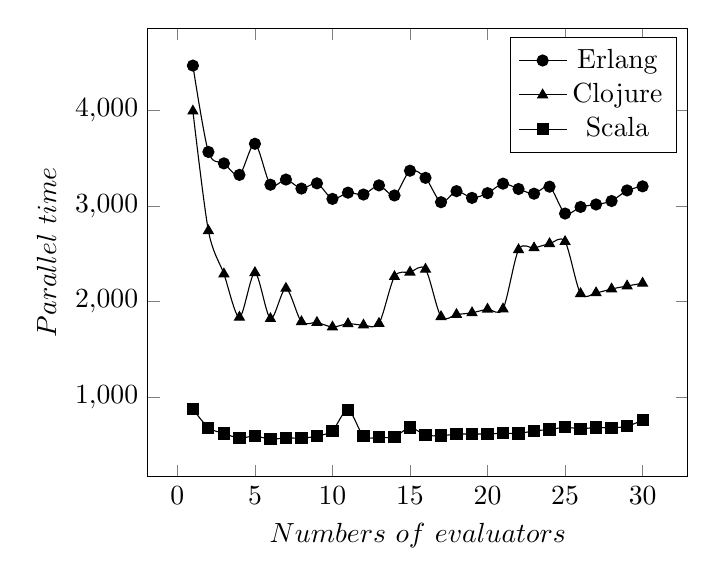
\begin{tikzpicture}

  \begin{axis}[
         xlabel=$Numbers \hspace{.12cm} of \hspace{.12cm} evaluators$,
         ylabel=$Parallel \hspace{.12cm} time$
         ]
     \addplot[smooth,mark=*]  plot coordinates{
(1,4466.6)
(2,3564.222222222222)
(3,3444.6666666666665)
(4,3324.5555555555557)
(5,3649.6)
(6,3221.7)
(7,3275.9)
(8,3181.3)
(9,3236.0)
(10,3073.5555555555557)
(11,3139.0)
(12,3119.1111111111113)
(13,3214.9)
(14,3109.5555555555557)
(15,3368.3)
(16,3293.7)
(17,3039.1)
(18,3154.7)
(19,3084.1)
(20,3133.6666666666665)
(21,3232.9)
(22,3177.1111111111113)
(23,3128.0)
(24,3201.3333333333335)
(25,2920.4)
(26,2989.5555555555557)
(27,3015.4)
(28,3051.4444444444443)
(29,3162.3)
(30,3204.7)
     };
     \addlegendentry{Erlang}

     \addplot[smooth,mark=triangle*]
         plot coordinates{
(1,3990.75)
(2,2740.777777777778)
(3,2289.1111111111113)
(4,1837.111111111111)
(5,2302.5555555555557)
(6,1822.6666666666667)
(7,2138.6666666666665)
(8,1789.5)
(9,1782.3333333333333)
(10,1734.6666666666667)
(11,1768.888888888889)
(12,1754.7777777777778)
(13,1772.0)
(14,2261.1111111111113)
(15,2307.8888888888887)
(16,2338.4444444444443)
(17,1842.3333333333333)
(18,1865.7777777777778)
(19,1883.4444444444443)
(20,1920.7777777777778)
(21,1923.5)
(22,2542.1111111111113)
(23,2561.6666666666665)
(24,2605.5555555555557)
(25,2627.0)
(26,2083.0)
(27,2091.8888888888887)
(28,2132.222222222222)
(29,2163.777777777778)
(30,2192.1111111111113)
         };
     \addlegendentry{Clojure}


     \addplot[smooth,mark=square*]
         plot coordinates{
(1,876.6666666666666)
(2,683.7777777777778)
(3,622.2857142857143)
(4,575.2222222222222)
(5,596.0)
(6,563.0)
(7,576.2222222222222)
(8,574.0)
(9,595.1111111111111)
(10,651.8888888888889)
(11,871.6666666666666)
(12,595.3333333333334)
(13,582.25)
(14,586.8888888888889)
(15,684.8888888888889)
(16,605.0)
(17,600.625)
(18,614.0)
(19,618.2222222222222)
(20,616.7777777777778)
(21,625.2222222222222)
(22,622.6666666666666)
(23,649.7777777777778)
(24,664.1111111111111)
(25,686.625)
(26,672.4444444444445)
(27,684.7777777777778)
(28,681.625)
(29,698.0)
(30,760.7142857142857)
         };
     \addlegendentry{Scala}

  \end{axis}

\end{tikzpicture}



\columnbreak
\item[] \textbf{Fig. 2.} Parallel running times for two reproducers.
    
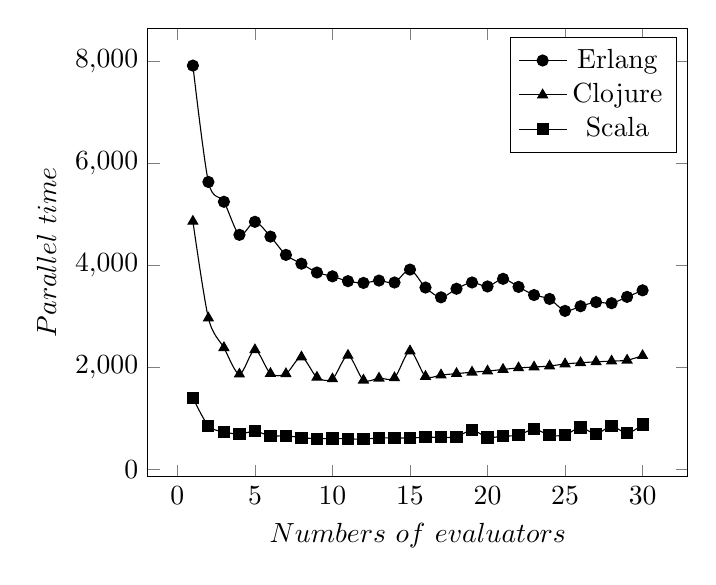
\begin{tikzpicture}

  \begin{axis}[
         xlabel=$Numbers \hspace{.12cm} of \hspace{.12cm} evaluators$,
         ylabel=$Parallel \hspace{.12cm} time$
         ]
     \addplot[smooth,mark=*]  plot coordinates{
(1,7919.428571428572)
(2,5638.0)
(3,5249.75)
(4,4601.5)
(5,4856.714285714285)
(6,4567.285714285715)
(7,4208.333333333333)
(8,4036.0)
(9,3862.777777777778)
(10,3788.3)
(11,3693.6)
(12,3659.2)
(13,3705.1111111111113)
(14,3667.0)
(15,3920.4)
(16,3568.2)
(17,3376.75)
(18,3544.7)
(19,3668.222222222222)
(20,3589.4)
(21,3739.222222222222)
(22,3580.9)
(23,3421.6)
(24,3345.222222222222)
(25,3110.8)
(26,3202.4)
(27,3282.1)
(28,3262.0)
(29,3385.4)
(30,3513.777777777778)
     };
     \addlegendentry{Erlang}

     \addplot[smooth,mark=triangle*]
         plot coordinates{
         (1,4866.5)
(2,2970.0)
(3,2389.5555555555557)
(4,1870.5555555555557)
(5,2347.1111111111113)
(6,1882.888888888889)
(7,1878.111111111111)
(8,2206.1111111111113)
(9,1808.4444444444443)
(10,1777.3333333333333)
(11,2238.1111111111113)
(12,1752.3333333333333)
(13,1791.888888888889)
(14,1798.888888888889)
(15,2324.777777777778)
(16,1825.7777777777778)
(17,1854.5555555555557)
(18,1881.5555555555557)
(19,1908.6666666666667)
(20,1931.5555555555557)
(21,1962.888888888889)
(22,1993.6666666666667)
(23,2010.111111111111)
(24,2030.5555555555557)
(25,2071.0)
(26,2094.3333333333335)
(27,2112.8888888888887)
(28,2126.4444444444443)
(29,2144.5555555555557)
(30,2233.222222222222)
         };
     \addlegendentry{Clojure}


     \addplot[smooth,mark=square*]
         plot coordinates{
(1,1406.8333333333333)
(2,854.5714285714286)
(3,741.0)
(4,694.75)
(5,752.2)
(6,660.1111111111111)
(7,663.4285714285714)
(8,626.5)
(9,605.375)
(10,609.125)
(11,602.7777777777778)
(12,596.1428571428571)
(13,620.8888888888889)
(14,619.7777777777778)
(15,619.0)
(16,634.2222222222222)
(17,631.8888888888889)
(18,641.8888888888889)
(19,775.5555555555555)
(20,630.625)
(21,656.6666666666666)
(22,672.7777777777778)
(23,796.2222222222222)
(24,671.1111111111111)
(25,679.3333333333334)
(26,825.8888888888889)
(27,696.2222222222222)
(28,854.5)
(29,711.0)
(30,882.6666666666666)
         };
     \addlegendentry{Scala}

  \end{axis}

\end{tikzpicture}



\end{itemize}
\end{small}
\end{multicols}

% \begin{multicols}{2}
% \begin{small}
% \begin{itemize}
% \item[] \textbf{Fig. 3.} Number of evaluators with best results for one reproducer.
%     \input{graphs/g2_1}

% \columnbreak
% \item[] \textbf{Fig. 4.} Number of evaluators with best results for two reproducers.
%     
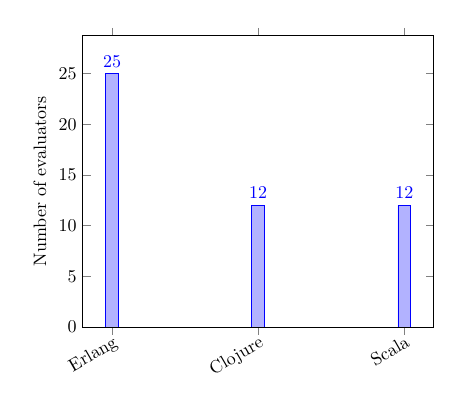
\begin{tikzpicture}[thick, scale=0.65]
  \begin{axis}[ybar,
    bar width=0.25cm,
    ymin=0,
    enlarge y limits={upper,value=0.15},
    legend style={at={(0.5,-0.25)},
    anchor=north,legend columns=-1},
    ylabel={Number of evaluators},
    symbolic x coords={Erlang, Clojure, Scala},
    xtick=data,
    xticklabel style={
        inner sep=0pt,
        anchor=north east,
        rotate=30
    },
    nodes near coords={\pgfmathprintnumber[fixed,precision=0]{\pgfplotspointmeta}},
    ]
    \addplot coordinates {(Erlang,25) (Clojure,12) (Scala,12)};
  \end{axis}
\end{tikzpicture}

% \end{itemize}
% \end{small}
% \end{multicols}

\begin{multicols}{2}
\begin{small}
\begin{itemize}
\item[] \textbf{Fig. 3.} Parallel time for 25 evaluators (Erlang's best case).
    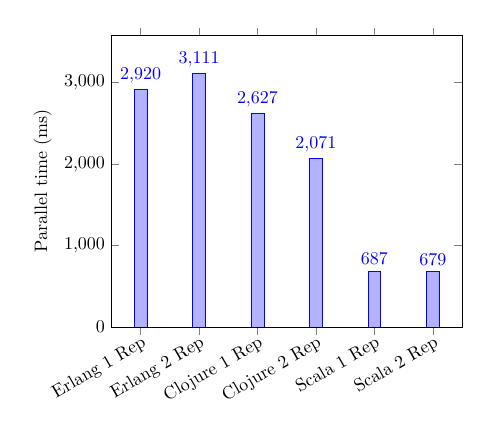
\begin{tikzpicture}[thick, scale=0.65]
  \begin{axis}[ybar,
    bar width=0.25cm,
    ymin=0,
    enlarge y limits={upper,value=0.15},
    legend style={at={(0.5,-0.25)},
    anchor=north,legend columns=-1},
    ylabel={Parallel time (ms)},
    symbolic x coords={Erlang 1 Rep, Erlang 2 Rep, Clojure 1 Rep, Clojure 2 Rep, Scala 1 Rep, Scala 2 Rep},
    xtick=data,
    xticklabel style={
        inner sep=0pt,
        anchor=north east,
        rotate=30
    },
    nodes near coords={\pgfmathprintnumber[fixed,precision=0]{\pgfplotspointmeta}},
    ]
    \addplot coordinates {(Erlang 1 Rep,2920.4) (Erlang 2 Rep,3110.8) (Clojure 1 Rep,2627) (Clojure 2 Rep,2071) (Scala 1 Rep,686.625) (Scala 2 Rep,679.3333333)};
  \end{axis}
\end{tikzpicture}

\columnbreak
\item[] \textbf{Fig. 4.} Parallel time for 10 evaluators (Clojure's best case).
    
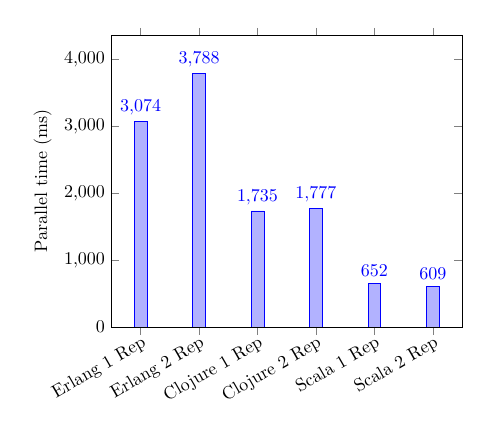
\begin{tikzpicture}[thick, scale=0.65]
  \begin{axis}[ybar,
    bar width=0.25cm,
    ymin=0,
    enlarge y limits={upper,value=0.15},
    legend style={at={(0.5,-0.25)},
    anchor=north,legend columns=-1},
    ylabel={Parallel time (ms)},
    symbolic x coords={Erlang 1 Rep, Erlang 2 Rep, Clojure 1 Rep, Clojure 2 Rep, Scala 1 Rep, Scala 2 Rep},
    xtick=data,
    xticklabel style={
        inner sep=0pt,
        anchor=north east,
        rotate=30
    },
    nodes near coords={\pgfmathprintnumber[fixed,precision=0]{\pgfplotspointmeta}},
    ]
    \addplot coordinates {(Erlang 1 Rep,3073.555556) (Erlang 2 Rep,3788.3) (Clojure 1 Rep,1734.666667) (Clojure 2 Rep,1777.333333) (Scala 1 Rep,651.8888889) (Scala 2 Rep,609.125)};
  \end{axis}
\end{tikzpicture}

\end{itemize}
\end{small}
\end{multicols}

Figures 1 and 2 show that the three languages had a good concurrent
behaviour: the overhead of manage more logical executing units than
the physical ones available didn't impact on the executing of the
algorithm, even when that number gradually increases.  
%
\setcounter{figure}{5}
%
\begin{figure}
\caption{Parallel time for 6 evaluators (Scala's best case).}
\centering
    
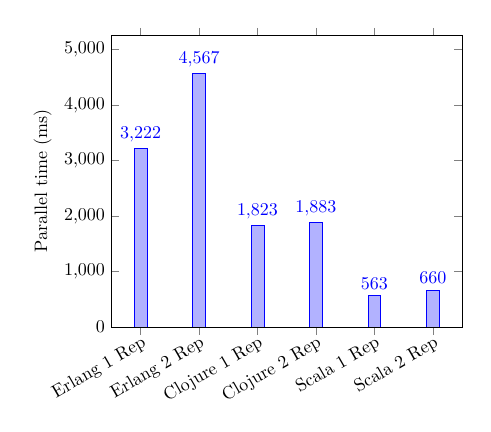
\begin{tikzpicture}[thick, scale=0.65]
  \begin{axis}[ybar,
    bar width=0.25cm,
    ymin=0,
    enlarge y limits={upper,value=0.15},
    legend style={at={(0.5,-0.25)},
    anchor=north,legend columns=-1},
    ylabel={Parallel time (ms)},
    symbolic x coords={Erlang 1 Rep, Erlang 2 Rep, Clojure 1 Rep, Clojure 2 Rep, Scala 1 Rep, Scala 2 Rep},
    xtick=data,
    xticklabel style={
        inner sep=0pt,
        anchor=north east,
        rotate=30
    },
    nodes near coords={\pgfmathprintnumber[fixed,precision=0]{\pgfplotspointmeta}},
    ]
    \addplot coordinates {(Erlang 1 Rep,3221.7) (Erlang 2 Rep,4567.285714) (Clojure 1 Rep,1822.666667) (Clojure 2 Rep,1882.888889) (Scala 1 Rep,563) (Scala 2 Rep,660.1111111)};
  \end{axis}
\end{tikzpicture}
\end{figure}

The Scala implementation are smoother in his results in contrast with
Clojure where many peaks were obtained. % Y habría que ver por qué - JJ
These two languages use the JVM
and the same random library, therefore there is a clear differences in
their concurrent models. The results for Scala and Clojure were better
with a small number of units of execution: when the number of evaluators
grows the efficiency of the algorithm falls. In this sense Erlang had
a non-typical behaviour,  improving up to 25 evaluators, only
then the speed began to decrease. 

Erlang was the language with the worst execution time; but its
runtime, in the best case, was able to schedule 52 units of execution
(far more than the others).  This fact point to a very particular way
of scheduling the process and must be studied more deply. Also the
speedup obtained relative to his sequential time is very good, this
two facts point to a possible good scalability. Clojure's performance
is medium, with a speedup close to $1$. 

Scala was the language with the best results, even when it's runtime are the same of Clojure's, his models of computation and concurrency (in particular his balance between mutable and immutable state) allow a better behaviour of the concurrent algorithms. Again is important to note the quality of the concurrent abstractions made by all this technologies in which the number of logical units of executions are greater than the number of the physical ones.

% Vaya follón quitar los números de figura automáticos... - JJ
Figures 3, 4, and 5 shows the results for 1 and 2 reproducers in the
cases of the number of evaluators 25, 10, and 6 which was the best
cases for each languages. These graphs confirms the differences in the
concurrent models of the technologies. 


\section{Conclusions}
\label{sec:conclusions}
    
This work shows the simplicity of the implementation  of a hybrid
parallel genetic algorithm in functional-concurrent languages. The
executions units were mapped to built-in concurrent concepts of languages
(actors and agents) and the procedural to functions or methods. 

Erlang and Clojure are languages that encourage a \emph{zero mutable
  state}-\emph{all functional} programming style with advantages in
the design an correction of the algorithms, The protocols of Clojure
allow the principles of OO without the complications of inheritance;
its concurrent concepts  are specialized and flexible at the same
time. The Scala language is multi-paradigm and hybrid in relation with
the computation modes supported. When a shared data structure is
needed this language allows a more direct access and that could be an
advantage, although this has not been shown in our experiments through
the scaling capability. 

Among the new trends in pGAs are new parallel platforms, the new
languages with concurrent abstractions build-in are parallel platforms
too, and their use for develop pGAs can be a very good approach for
new GA developments. In the pGA model used in this work the chosen GA
architecture are concurrent-rich but the implementation remains simple
thanks of the high level of abstraction of the implementation
technologies. This paper is a proof of concept on how to map EAs to
these architectures, but at the same time show the strength and
weaknesses of each implementation. Generally speaking, Java based
languages such as Clojure and Scala are faster that Erlang running its
own virtual machine, but Erlang shows superior scalability which, in
certain scenarios, could mean that it could achieve better solutions
than the other two. 

We have also tested the scalability of the implementations in a
pool-based implementation, which shows the limitations of such
architectures; however, no attempt has been made to optimize it so the
only qualitative conclusion we can draw is that Erlang shows the best
scalability; that only one reproducer offers better results than two
in all cases, and that a good thing about these languages is that
performance does not suffer, but degrades gracefully, when many
threads are running at the same time. 

Our experiments shows Scala's performance like the best and point to Erlang like an very scalable runtime, the recommendations are to enrich the experiments with more complex case of study and to test the libraries in heterogeneous hardware in order to check scalability of each language.



%ACKNOWLEDGMENTS are optional
%\section{Agradecimientos}
%
%Este trabajo se está desarrollando gracias a la financiación de  los proyectos EvOrq (P08-TIC-3903), CANUBE (CEI2013-P-14) y ANYSELF (TIN2011-28627-C04-02). Es también respaldado por el Programa de Doctorado de la AUIP y por el proyecto 83 del Campus CEI BioTIC.


\bibliographystyle{splncs}
\bibliography{osgiliath,geneura,referencias,erlang-ae-model}

\end{document}

